% RQ3
\newpage
\section{Ranking}
\label{sec:toolranking}
% Most important:
% Finding the top performing tool is most important, then low MSE for that top performing
% Confidence in automation
% 
Following the performance prediction as described in the previous section, the methodology to answer research question 3: \textit{Is it possible to generate a ranking of tools according to their performance on unseen datasets?}; 

will be covered. An estimator for future error detection tool performance was introduced in the previous section. Now, the goal of an generating an estimated ranking of tools with respect to their performance will be discussed.
~\\An absolute score is helpful to know with a single tool at your disposal, but a ranking or recommendation of tools and their strategies would be of greater use for the end-user. The question proposed here is to see if such a ranking could be made, ranking the better performing tools higher in the ranking. 
The flow of creating such a ranking is shown in \autoref{fig:method_ranking}. For a new dataset as input, all the estimators will give an estimation of what the performance score on that new dataset will be. These estimations will then be ordered into a ranking, with the estimated highest performing strategies on top and worst estimated performing strategies on the bottom. A user could then make a substantiated choice for which error detection strategy to choose, based on expected performance.

\begin{figure}[h]
    \centering
    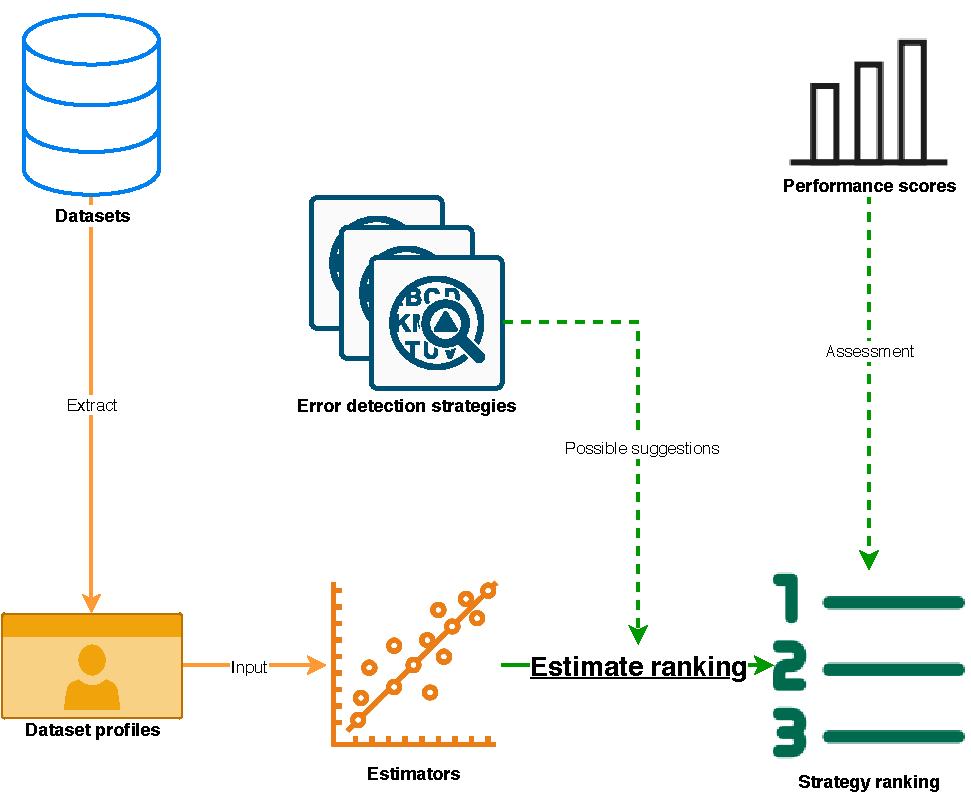
\includegraphics[width=0.9\textwidth]{thesis/Figures/Method/PerformanceEstimation-Ranking.pdf}
    \caption{Flow of the estimation of strategy ranking}
    \label{fig:method_ranking}
\end{figure}

\subsection{Method of ranking}
A user should be able to retrieve an estimated ranking of high performing strategies without running these tool on an unseen dataset. A ranking should be $K$ strategies long, with a predefined $K$. It should be so that a user can a variety of tools and configurations to pick from. To evaluate whether it is possible to create such an estimated ranking, two types of rankings will be made and scored. First, a ranking based on finding the \textbf{best tool} for the dataset will be created. Then, a ranking based on finding the \textbf{best configuration for a tool} will be created.
To test if estimated strategy ranking is viable, this section will focus on F1 estimation and ranking. 
\\To generate an estimated ranking for a new unseen dataset, the data profile as described in \autoref{subsec:dataprofiles} is created. Then, all estimators as found by \autoref{subsec:estimatorselection} are given this data profile as input, generating estimated scores for all strategies $s \in S$. These estimated scores (like a single column in \autoref{tab:estimatedscores}) are then sorted. Depending on the task (best tool or best configuration), the results are filtered and only the top suggestions are kept.

\paragraph{Best tool} First, the ranking of the best tool for a dataset will be discussed. This is the use case where a user does not know which tool he or she wants to use. The tools will be ranked according to the estimated performance score, with one output row per tool. An example of such a ranking is shown in \autoref{tab:ranking_best_tool}. In this example, there are 6 error detection tools available, just like the 6 tools that are used in this research. In the "Tool" column, it is shown which tool is suggested at that ranking. Also in this ranking, the estimated best configuration for that tool will be suggested in the "Configuration". Lastly, the predicted F1 score will be shown for comparison of predicted performances of the strategies. A user will be able to choose an error detection strategy directly from this list.

\begin{table}[h]
\centering
\begin{tabular}{|l|l|l|l|}
\hline
\textbf{Rank} & \textbf{Tool} & \textbf{Configuration} & \textbf{Estimated F1} \\ \hline
1             & Tool 1        & Config 1-a             & $\hat{y}(s_{1-a}, d)$ \\ \hline
2             & Tool 2        & Config 2-a             & $\hat{y}(s_{2-a}, d)$ \\ \hline
3             & Tool 3        & Config 3-a             & $\hat{y}(s_{3-a}, d)$ \\ \hline
4             & Tool 4        & Config 4-a             & $\hat{y}(s_{4-a}, d)$ \\ \hline
5             & Tool 5        & Config 5-a             & $\hat{y}(s_{5-a}, d)$ \\ \hline
6             & Tool 6        & Config 6-a             & $\hat{y}(s_{6-a}, d)$ \\ \hline
\end{tabular}
\caption{Strategy ranking for best tool}
\label{tab:ranking_best_tool}
\end{table}

\paragraph{Best configuration per tool} Another ranking that could be made, is a configuration ranking per tool, for a specific dataset. An example of this ranking is shown in table. \autoref{tab:ranking_best_configuration}. It might happen that a user has decided to work with a specific tool. However, the user is not aware of the best configuration for that tool. So, for one single tool, $K$ different configurations will be outputted in a ranking. The format of the ranking will be the same as the "best tool" ranking, but only 1 tool type will be shown. As shown in the \autoref{tab:ranking_best_configuration}, in column "Tool", only 1 tool is selected. Then, in column "Configuration", the different configurations will be ordered from best to worst. Again, the predicted performance score will be displayed in the last column in descending order. 

\begin{table}[h]
\centering
\begin{tabular}{|l|l|l|l|}
\hline
\textbf{Rank} & \textbf{Tool} & \textbf{Configuration} & \textbf{Estimated F1} \\ \hline
1             & Tool 1        & Config 1-a             & $\hat{y}(s_{1-a}, d)$ \\ \hline
2             & Tool 1        & Config 1-b             & $\hat{y}(s_{1-b}, d)$ \\ \hline
3             & Tool 1        & Config 1-c             & $\hat{y}(s_{1-c}, d)$ \\ \hline
4             & Tool 1        & Config 1-d             & $\hat{y}(s_{1-d}, d)$ \\ \hline
5             & Tool 1        & Config 1-e             & $\hat{y}(s_{1-e}, d)$ \\ \hline
6             & Tool 1        & Config 1-f             & $\hat{y}(s_{1-f}, d)$ \\ \hline
7             & Tool 1        & Config 1-g             & $\hat{y}(s_{1-g}, d)$ \\ \hline
8             & Tool 1        & Config 1-h             & $\hat{y}(s_{1-h}, d)$ \\ \hline
9             & Tool 1        & Config 1-i             & $\hat{y}(s_{1-i}, d)$ \\ \hline
10            & Tool 1        & Config 1-j             & $\hat{y}(s_{1-j}, d)$ \\ \hline
\end{tabular}
\caption{Strategy ranking for best configuration per tool}
\label{tab:ranking_best_configuration}
\end{table}

\subsection{Performance measure of ranking}
% To analyze the results of the produced rankings, the ranked strategies of first will be qualitatively be addressed. Generating actual lists of suggested error detection strategies to use and glancing over them will give a first indicates on whether the results will be promising.
Quantitative metrics will be calculated to compare and analyze the results of these rankings.
Average Precision is a metric that takes into account the ranking of the returned documents. Unfortunately, this metric uses a binary relevance scoring, where the last relevant document is equally important to rank high as the first relevant document. In this research, a cutoff point for a score should then be chosen to evaluate, for example, any strategy with a score > 0.5 would be considered relevant. Taking the mean average precision for all different unseen datasets and the produced rankings would then have some meaning, but does not fit this purpose best.

~\\A metric that does take the relative importance into account, is the discounted cumulative gain (DCG). It allows degrees of relevance, which is suited for our purpose. The top ranks count the most, meaning whenever a highly relevant (high scoring strategy) is actually listed at the top, the DCG reflects that in a positive way. The utility also decreases with the rank, meaning that lower ranks count less towards the DCG. The DCG is a summation of the relevance score discounted by a log value relative to the given place in the ranking (shown in \autoref{eq:DCG}).
~\\Also, a normalized version of the discounted cumulative gain exists. It takes the ideal ranking and calculates the DCG ($IDCG_k$). The output metric will be the $DCG_k$ for the produced ranking, divided by the DCG for the best ranking (see \autoref{eq:NDCG}). 

\begin{equation}
\label{eq:DCG}
    DCG_k = \sum^k_{r=1} \frac{rel_r}{\log(r+1)}
\end{equation}

\begin{equation}
\label{eq:NDCG}
    NDCG_k = \frac{DCG_k}{IDCG_k}
\end{equation}

The relevance of a returned item in a ranking must be determined beforehand. It should have a relation to how good a strategy performs. 
That is why for this research, the actual real score (precision, recall or F1) of a strategy run on a specific dataset will be the relevance. This allows this for automatic relevance scoring. As shown in \autoref{fig:method_ranking} and as described in the previous sections, it is possible to assess the produced strategy ranking by using real performance scores from the empirical study as relevance.


\paragraph{Best tool ranking scoring} The best tool ranking will be scored in two ways. When a ranking like displayed in \autoref{tab:ranking_best_tool} is given, scoring can be done tool-wise, but also strategy-wise. The first way is to get the highest relevance for all the configurations of that tool and using that value as $rel_r$. This will judge a ranking solely on the order of tools given. The second way of ranking will be taking the relevance of the suggested strategy for scoring. This is a more difficult task for the recommendation system, as not only does the tool suggestion need to be correct, but the only configuration for that tool should also be the best configuration. 

\subsection{Evaluation}
Again, similarly to \autoref{sec:performanceprediction}, the experiments as proposed above will be assessed qualitatively and quantitatively to answer the third research question: \textit{Is it possible to generate a ranking of tools according to their performance on unseen datasets?}; 

~\\In total 3 types of experiments will be conducted. 
\begin{itemize}
    \item Best tool ranking - Scored on tool + configuration relevance
    \item Best tool ranking - Scored on tool relevance
    \item Best configuration ranking - Scored on configuration relevance
\end{itemize}

The estimated rankings will be produced using leave-one-out cross validation, like in \autoref{sec:performanceprediction}. 

For the first two types of experiments, the same rankings are used. These rankings will consist of 6 entries ($K = 6$), namely for the 6 possible tools to be suggested. 
For the last type of experiments, the rankings will consist of 10 suggestions\footnote{For this research, a $K$ of 10 will be used. 10 is the number of search suggestion in the basic Google search bar (\url{https://www.google.com/}).} ($K = 10$) of configurations for a tool. Therefore, only tools with 10+ configurations will be tested in this experiment (dBoost \& Raha), as this will test the capability of the ranking system to produce the right order of ranking, but also cutting off the majority of configurations.

For each dataset, the ranking will be scored with NDCG, using the best possible ranking from the ground truth as a reference ideal DCG score. This will result in a NDCG for all datasets available. These scores will the main subject of analysis for evaluation.

\paragraph{Qualitative} The NDCG values per dataset for each experiment will be sorted and plotted for comparison. The focus of the qualitative analysis will be that of the ordering and general relative results between datasets in one experiment. Preferably, NDCG values per dataset are similarly high, without many lower outliers. If there is a cluster of lower NDCG values, the ranking will be deemed meaningless.

\paragraph{Quantitative} Similar to \autoref{sec:performanceprediction}, the results of the experiments will be compared to a baseline method. This baseline method estimates performance as described in \autoref{subsec:evaluation_performanceprediction}. From these baseline estimation, rankings of the same structure as in the experiments will be created and scored with NDCG. While the focus lies on the F1-score for this section, a comparison of mean NDCG for all datasets will be compared for precision based ranking, recall based ranking and F1 based ranking, both directly estimated and combinedly estimated (recall + precision estimation to calculate the estimated F1).

The main comparison to answer if it possible to generate a ranking of tools according to their performance on unseen datasets, will be to see if there is an increase in the mean NDCG for all experiments from the proposed estimator compared to the baseline, described in the paragraph above. If there is no increase in NDCG, the estimator will be deemed not suitable for estimated strategy ranking. 